%==============================================================================
% Voorbeeld gebruik documentklasse hogent-article
%==============================================================================
%
% Compileren in TeXstudio:
%
% - Zorg dat Biber de bibliografie compileert (en niet Biblatex)
%   Options > Configure > Build > Default Bibliography Tool: "txs:///biber"
% - F5 om te compileren en het resultaat te bekijken.
% - Als de bibliografie niet zichtbaar is, probeer dan F5 - F8 - F5
%   Met F8 compileer je de bibliografie apart.
%
% Als je JabRef gebruikt voor het bijhouden van de bibliografie, zorg dan
% dat je in ``biblatex''-modus opslaat: File > Switch to BibLaTeX mode.

\documentclass{hogent-article}

\usepackage{lipsum} % Voor vultekst
\usepackage{graphicx}
\usepackage{float}
\graphicspath{ {./img/} }

%------------------------------------------------------------------------------
% Metadata over het artikel
%------------------------------------------------------------------------------

%---------- Titel & auteur ----------------------------------------------------

% TODO: geef werktitel van je eigen voorstel op
\PaperTitle{Zijn mensen die uit een succesvol gezin komen meer wiskundig geletterd dan mensen die uit minder succesvolle gezinnen komen?}
% TODO: geef op welk soort artikel dit is
% Dit is typisch de opdracht en het vak waarvoor dit artikel geschreven is, bv.
% ``Verslag onderzoeksproject Onderzoekstechnieken 2018-2019''
\PaperType{Verslag NPE-opdracht Research Techniques 2020-2021}

% TODO: vul je eigen naam in als auteur, geef ook je emailadres mee!
\Authors{Vic Rottiers\textsuperscript{1}, Pieter Van Keer\textsuperscript{2}, Nicolas De Wree\textsuperscript{3}, Brent De Craemer\textsuperscript{4}} % Authors

% TODO: vul de naam van je co-promotor in.
% Als het hier gaat om een voorstel voor de bachelorproef, dan ben je hier
% verplicht de naam van je co-promotor in te vullen. Zoniet, dan kan je het
% leeg laten.
\CoPromotor{}

% Contactinfo: Geef hier de contactgegevens van elke auteur van het artikel (en
% indien van toepassing ook van de co-promotor).
\affiliation{
  \textsuperscript{1} \href{mailto:vic.rottiers@student.hogent.be}{vic.rottiers@student.hogent.be}}
\affiliation{
  \textsuperscript{2} \href{mailto:pieter.vankeer@student.hogent.be}{pieter.vankeer@student.hogent.be}
}
\affiliation{
    \textsuperscript{3} \href{mailto:nicolas.dewree@student.hogent.be}{nicolas.dewree@student.hogent.be}
}
\affiliation{
    \textsuperscript{4} \href{mailto:brent.decraemer@student.hogent.be}{brent.decraemer@student.hogent.be}
}

%---------- Abstract ----------------------------------------------------------

\Abstract{In een constant evoluerende wereld heeft elk gevolg een oorzaak. Het is belangrijk dat we onderliggende oorzaken vinden om ze te kunnen begrijpen en er te kunnen op inspelen. Om meer mensen te hebben met een hoge wiskundige geletterdheid moeten we eerst de oorzaak vinden die leidt naar een verbeterde wiskundige geletterdheid. Kan je wiskundige geletterdheid overerven van je ouders? Ben je meer wiskundig geletterd als je ouders meer financiële middelen hebben? Dit werk is noodzakelijk naar de toekomst toe als we het algemeen niveau van wiskundige geletterdheid willen laten stijgen.
}

%---------- Onderzoeksdomein en sleutelwoorden --------------------------------
% TODO: Vul de sleutelwoorden aan.


\Keywords{Wiskundige geletterdheid bij studenten van HoGent; Wiskundige geletterdheid;}
\newcommand{\keywordname}{Sleutelwoorden} % Defines the keywords heading name

%---------- Titel, inhoud -----------------------------------------------------

\begin{document}

\flushbottom % Makes all text pages the same height
\maketitle % Print the title and abstract box
\tableofcontents % Print the contents section
\thispagestyle{empty} % Removes page numbering from the first page

%------------------------------------------------------------------------------
% Hoofdtekst
%------------------------------------------------------------------------------

\section{Inleiding}

Jarenlang is er veel discussie geweest over het belang van wiskunde in de informatica. 
Sommigen geloven dat het slechts weinig waarde toevoegt binnen de computerwetenschappen, terwijl anderen denken dat het essentieel is voor het vakgebied. 
Wij gaan onderzoeken of er factoren zijn die de mate waarin je wiskunde beheerst beïnvloeden. De enquête is afgenomen bij studenten in het tweede jaar bachelor Toegepaste informatica aan de Hogeschool van Gent, meer hierover kan u lezen bij de Methodologie. 

\begin{quote}Zijn mensen die uit een succesvol gezin komen meer wiskundig geletterd dan mensen die uit minder succesvolle gezinnen komen?\end{quote}

We gaan onderzoeken of de graad van succes van het gezin / de ouders invloed heeft op hoe wiskundig geletterd de kinderen zijn.
Onder succes verstaan we dat de ouders een hoog diploma hebben, dus een master opleiding of bachelor opleiding gevolgd hebben. Alsook bepaalt het inkomen en de werkfunctie van de ouders het succes van het gezin.

Als groep denken we dat de succesgraad van het gezin een bepaalde positieve invloed heeft op de wiskundige geletterdheid van de kinderen.

\section{Overzicht literatuur}

% Refereren naar de literatuur kan met:
% \autocite{BIBTEXKEY} -> (Auteur, jaartal)
% \textcite{BIBTEXKEY} -> Auteur (jaartal)
Wiskundige geletterdheid is de competentie van het verwerven en verwerken van wiskundige informatie, alsook het gericht kunnen gebruiken van die informatie binnen de wiskunde.

Uit de 8 publicaties blijkt dat er factoren de wiskundige geletterdheid beïnvloeden. Een paar voorbeelden van factoren die worden aangehaald in de publicaties zijn de volgende: ouders, omgeving, school, vrienden, manier van leren, ... \autocite{Sosnowski2017}

Er zijn ook publicaties \autocite{Brum2007} die vermelden dat wiskundige geletterdheid niet enkel van de schoolbanken afkomstig is (school based), maar ook van thuis uit of bij vrienden wordt dit beïnvloed. Realistischere oefeningen en voorbeelden tijdens het aanleren van nieuwe begrippen zorgt er ook voor dat studenten dit sneller oppikken, en dit sneller volledig begrijpen \autocite{Vithal2006}.  


Andere artikels suggereren dat door het beginnen met aanleren van wiskundige concepten op jongere leeftijd een positieve invloed heeft op het kind. Zo kan het kind als het ouder wordt beter studeren, en beter nieuwe concepten begrijpen en toepassen \autocite{Vrijmoeth2010}. Angst voor wiskundige is ook een andere factor die de wiskundige geletterdheid kan beïnvloeden. Zo kan een student logisch gezien in staat zijn wiskundige concepten zeer goed te begrijpen en toe te passen, maar lukt hem/haar dit niet doordat er zich een angst voor wiskunde heeft ontwikkeld \autocite{Joseph2017}. Deze angst kan zich ontwikkelen door een trauma dat zich in het verleden voordeed. 



\section{Methodologie}

In het academiejaar 2019 - 2020 hebben de studenten van het vak onderzoekstechnieken aan de Hogeschool Gent data verzamelt rond het onderwerp wiskundige geletterdheid. Dit heeft men op verschillende wijze gedaan. De studenten namen deel aan een toets die naar de wiskundige geletterdheid peilt. Zo kon men een initiële indruk opvangen van wat voor data men kon verwachten bij het opstellen van de enquête, en zo kan men deze data gebruiken als input voor de analyse. Na het analyseren van de data heeft men verschillende hypotheses opgesteld, en aan de hand van deze hypotheses kon men de vragen van de enquête opstellen. Deze enquête bevatte verschillende vragen, en had als doel het verzamelen van data zodat hier verdere analyses op konden uitgevoerd worden.

Na het verzamelen werd als laatste stap alle data van het onderzoek geanonimiseerd door de begeleiders, en werd deze grote dataset doorgegeven aan ons, zodat wij deze data verder konden onderzoeken e analyseren. 


Als eerste stap hebben we als team ons ingewerkt in het onderwerp. Er werd research verricht naar het wiskundige geletterdheid, met als doel te achterhalen welke onderzoeken er al reeds werden uitgevoerd en wat de resultaten uit dit onderzoek bleken te zijn. Dit was anderzijds ook een zeer interessante bron om later onze conclusies uit ons eigen onderzoek te trekken. Dit is een goede maatstaf om na te gaan of het onderzoek realistisch is in vergelijking met de soortgelijke onderzoeken die men reeds had uitgevoerd.

Vervolgens gingen we aan de slag met de dataset, en onderzochten we welke variabelen een interessante keuze waren. Nadien stelden we dan ook onze onderzoeksvraag en op baseerde we onze hypothese op de opgezochte informatie die we vergaard hadden.

Eens we de hypothese opgesteld hadden werd er een Reading Group gehouden, zodat we onze opgezochte informatie konden bespreken en vergelijken met elkaar. Op deze manier controleren we elkaars werk, alsook wordt de informatie met elk groepslid gedeeld. Als voorlaatste en laatste stap werkten we de analyse uit, en werd het rapport gefinaliseerd. De analyse werd aan de hand van T-testen uitgevoerd, waar we voor elk verband van variabelen dit getest hebben en vervolgens onze bevindingen gerapporteerd hebben. 


\section{Experimenten}
De dataset bevat zoals reeds uitgelegd in \textbf{Methodologie } de resultaten van de enquête die in het academiejaar 2019 - 2020. De analyse hebben we uitgevoerd doormiddel van paren te maken van kwantitatieve en kwalitatieve variabelen. Op deze paren voerden we een rechtszijdige T-test uit, alsook het berekenen van cohens-d. Uit deze resultaten leidde we af of dit paar een verband had, alsook hoe sterk dit verband is.


\section{Analyse resultaten}

De statistische analyse over dit onderzoek kan u bekijken in de map /analyse.
Hier is te zien hoe er wel degelijk een verband is tussen de punten die leerlingen scoren op een bepaald olod en het diploma van hun ouders. Bijvoorbeeld scoorden kinderen waar de vader een master diploma of dergelijke had hoger op het olod Math4IT dan kinderen die ouders hebben met een lager secundair diploma. Zie Figuur \ref{fig:gradeMath4IT-EducationFather}.

\begin{figure}[h!]
    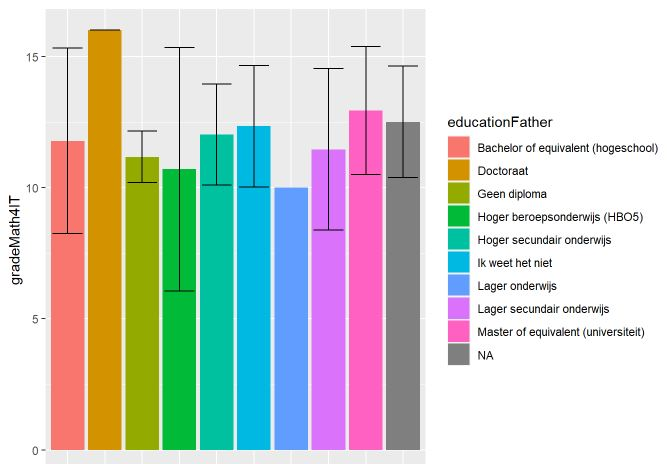
\includegraphics[width=\linewidth]{gradeMath4IT-EducationFather.JPG}
    \caption{Het verband tussen de punten van Math4IT en het diploma van de vader.}
    \label{fig:gradeMath4IT-EducationFather}
\end{figure}
%%Bij moeder is dit gelijkaardig. \ref{fig:gradeMath4IT-EducationMother}
\begin{figure}[h!]
    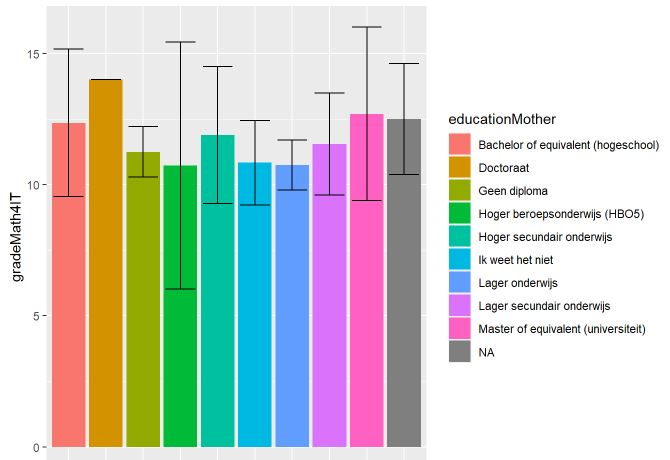
\includegraphics[width=\linewidth]{gradeMath4IT-EducationMother.JPG}
    \caption{Het verband tussen de punten van Math4IT en het diploma van de moeder.}
    \label{fig:gradeMath4IT-EducationMother}
\end{figure}

Over het algemeen hebben de ouders meer invloed op de punten van Math4IT dan de punten op Probleemoplossend denken I. Zie figuur \ref{fig:gradePOD-EducationFather}
\begin{figure}[H]
    \includegraphics[width=\linewidth]{gradePOD-EducationFather.JPG}
    \caption{Het verband tussen de punten van Probleemoplossend denken en het diploma van de vader.}
    \label{fig:gradePOD-EducationFather}
\end{figure}
\begin{figure}[h!]
    \includegraphics[width=\linewidth]{gradePOD-EducationMother.JPG}
    \caption{Het verband tussen de punten van Probleemoplossend denken en het diploma van de moeder.}
    \label{fig:gradePOD-EducationMother}
\end{figure}

Het inkomen van de ouders heeft weinig tot geen invloed op de prestaties van hun kinderen. Dit kan te danken zijn aan de mogelijkheden die de overheid ter beschikking stelt, Denk aan beurzen en studietoelagen. Zie figuur \ref{fig:gradeMath4IT-FamilyIncome} en \ref{fig:gradePOD-FamilyIncome}
\begin{figure}[h!]
    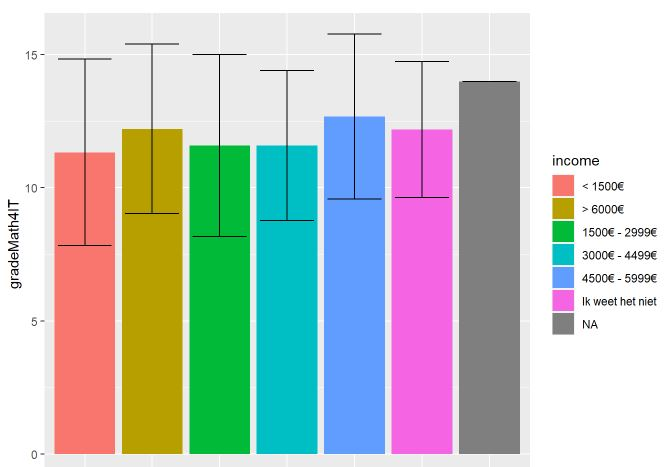
\includegraphics[width=\linewidth]{gradeMath4IT-FamilyIncome.JPG}
    \caption{Het verband tussen de punten van Math4IT en het inkomen van het gezin.}
    \label{fig:gradeMath4IT-FamilyIncome}
\end{figure}
\begin{figure}[h!]
    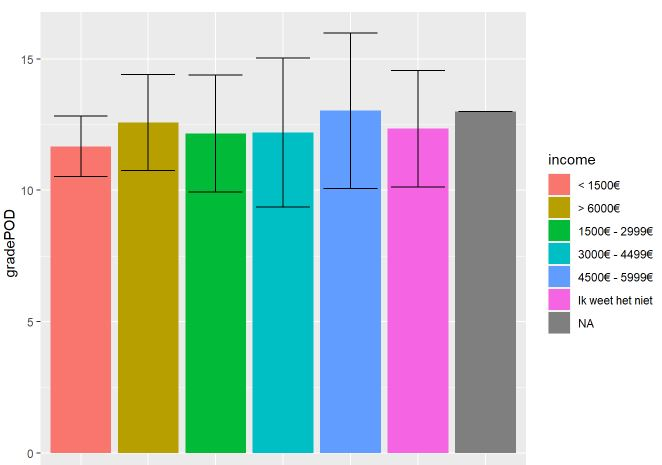
\includegraphics[width=\linewidth]{gradePOD-FamilyIncome.JPG}
    \caption{Het verband tussen de punten van Probleemoplossend denken en het inkomen van het gezin.}
    \label{fig:gradePOD-FamilyIncome}
\end{figure}

Uit de resultaten van de analyse over de functie van de ouders en de punten van de kinderen kunnen we concluderen dat er wel degelijk een verband is. Hier is te zien dat de punten van kinderen, met ouders die werkloos zijn, een stuk lager liggen dan kinderen waarvan de ouders wel gaan werken. Zie figuur \ref{fig:gradeMath4IT-OccupationFather}, \ref{fig:gradeMath4IT-OccupationMother}, \ref{fig:gradePOD-OccupationFather} en \ref{fig:gradePOD-OccupationMother}

Over het algemeen merken we, in de testen, dat de vader een grotere invloed heeft op de resultaten dan de moeder.
\begin{figure}[h!]
    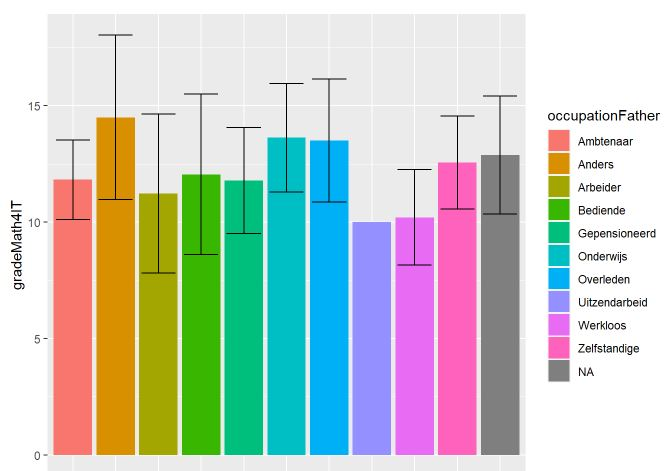
\includegraphics[width=\linewidth]{gradeMath4IT-OccupationFather.JPG}
    \caption{Het verband tussen de punten van Math4IT en de functie van de vader.}
    \label{fig:gradeMath4IT-OccupationFather}
\end{figure}
\begin{figure}[h!]
    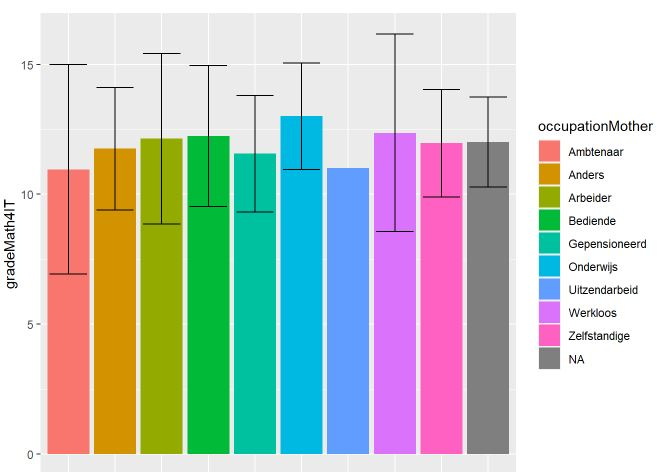
\includegraphics[width=\linewidth]{gradeMath4IT-OccupationMother.JPG}
    \caption{Het verband tussen de punten van Math4IT en de functie van de moeder.}
    \label{fig:gradeMath4IT-OccupationMother}
\end{figure}
\begin{figure}[h!]
    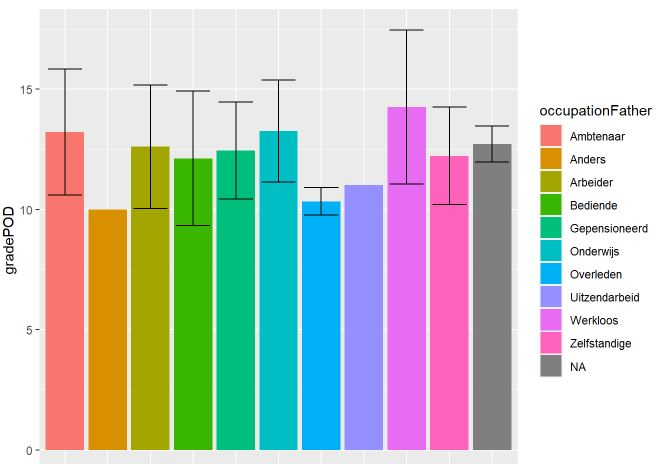
\includegraphics[width=\linewidth]{gradePOD-OccupationFather.JPG}
    \caption{Het verband tussen de punten van Probleemoplossend denken en de functie van de vader.}
    \label{fig:gradePOD-OccupationFather}
\end{figure}
\begin{figure}[h!]
    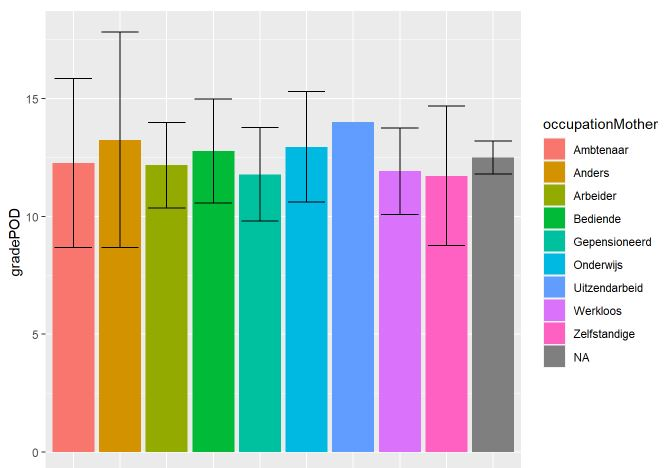
\includegraphics[width=\linewidth]{gradePOD-OccupationMother.JPG}
    \caption{Het verband tussen de punten van Probleemoplossend denken en de functie van de moeder.}
    \label{fig:gradePOD-OccupationMother}
\end{figure}

\section{Conclusie}
Uit de analyse resultaten valt op dat er geen concreet eenvoudig antwoord is op onze onderzoeksvraag. Er zijn weldegelijk factoren van de ouders die de wiskundige geletterdheid beïnvloeden, maar niet elke factor die onderzocht werd blijkt dit stramien te volgen. Voorbeelden hiervan vind u terug in de analyser resultaten hierboven. 

Hierbij kunnen we concluderen dat de hypothese die opgesteld was noch juist, noch fout is. Er zijn bepaalde factoren die een invloed vertonen, en andere factoren die geen verband blijken te hebben.

%------------------------------------------------------------------------------
% Referentielijst
%------------------------------------------------------------------------------
% TODO: de gerefereerde werken moeten in BibTeX-bestand ``bibliografie.bib''
% voorkomen. Gebruik JabRef om je bibliografie bij te houden en vergeet niet
% om compatibiliteit met Biber/BibLaTeX aan te zetten (File > Switch to
% BibLaTeX mode)

\phantomsection
\printbibliography[heading=bibintoc]

\end{document}
